\section{Ongoing work} % or "Research Plan"
\label{sec:vis}

Our ultimate goal is to build infrastructure to enable civil engineers to visually compare these multi-variate temporal data. In collaboration with the domain experts, we arrived at the following visualization tasks:
\begin{itemize}
	\item [T1]  Summarize all the earthquakes simulations to help engineers make scientific and quantitative comparisons between them; 
	\item [T2] For a specific earthquake simulation, explore the multivariate data and spot interesting patterns;
	\item [T3] When an interesting event is identified, obtain similar events on other simulations, so the context in which these events happened can be compared.
	%%\item [T1] An overview which summarizes all the earthquake simulations and can help them spotting outliers;
	%%\item [T2] For a specific earthquake simulation, a context view to explore the multivariate dataset and help engineers find interesting patterns across time;
	%%\item [T3] For the two views above, build efficient navigation and interaction between them;
        %%\item [T4] When an interesting event is identified, it should be possible to find similar events on other simulations, so the context in which these events happened can be compared.
\end{itemize} 


%% \subsection{Data Structure}
%% \label{sec:data}
%% \begin{figure}[h]
%% 	\centering % avoid the use of \begin{center}...\end{center} and use \centering instead (more compact)
%% 	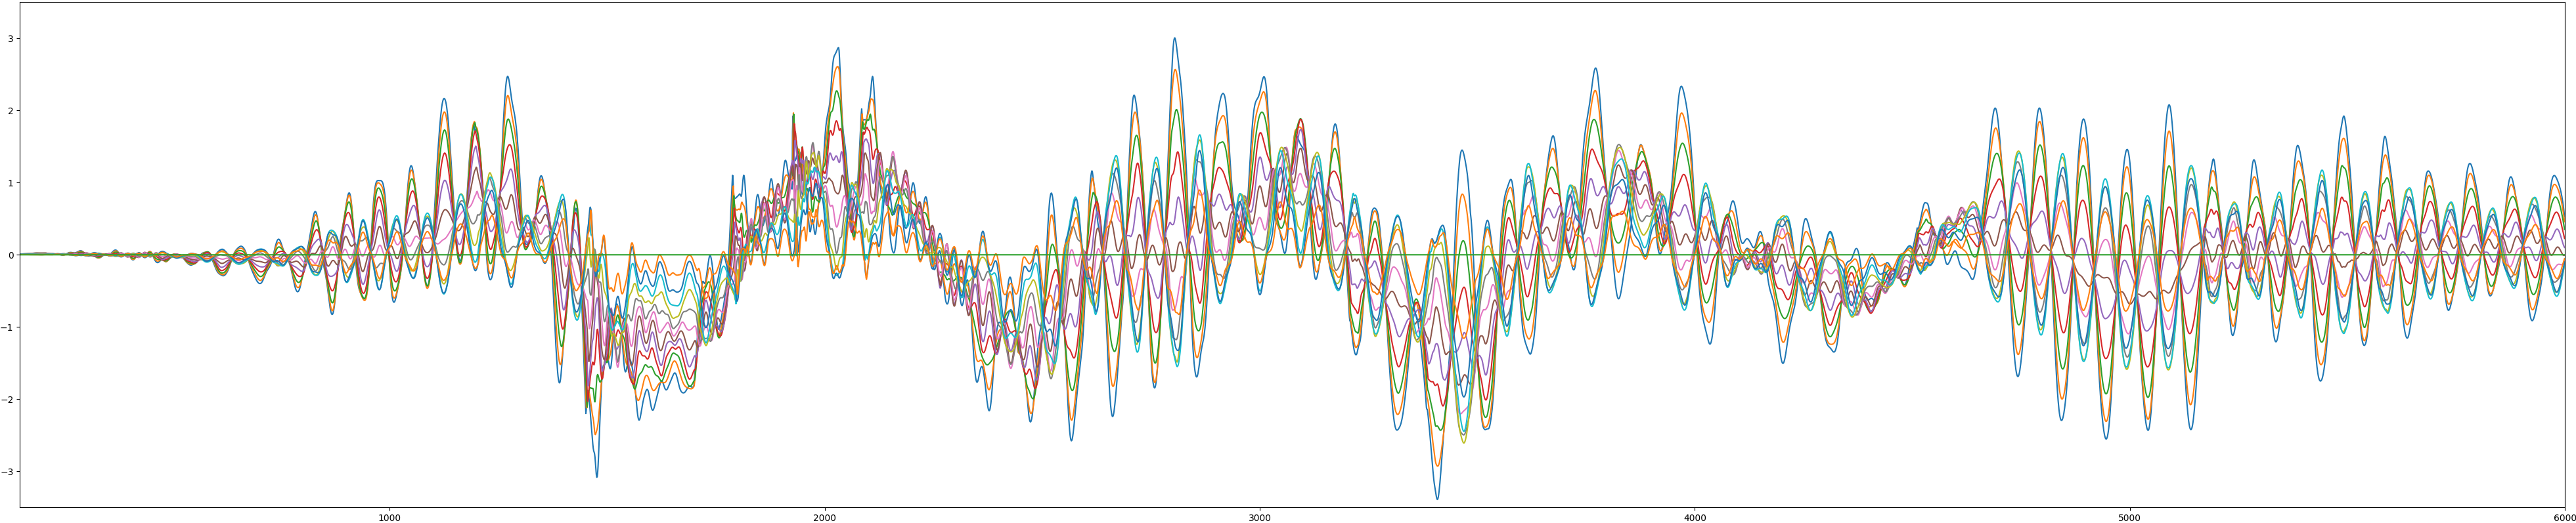
\includegraphics[width=\columnwidth]{figs/eq} 
%% 	\caption{time series for "Shear" attribute of one earthquake simulation}
%% 	\label{fig:data}
%% \end{figure}

Towards this end, we built a prototype interface using 50 of the available earthquake simulations.
The simulations track 6 physical attributes of interest, for each floor: acceleration, shear, diaphragm force, moment, drift ratio, and interstory drift ratio. For example, shear measures the stress parallel to each floor, while interstory drift ratio measures the positional difference between two adjacent floors at a given point in time. 
This gives a vector-valued time series for each attribute, and each simulation has $25,000$ time steps in average.
Each attribute is normalized by dividing the raw value by a predetermined design limit. This has the benefit that any value of the time series above 1 or below negative 1 indicate that the building is operating out of its safe design specifications, and mitigates the issue of comparing variables of different units.

\paragraph*{Implementation details}
The current prototype is implemented in Javascript using D3~\cite{Bostock:2011:DDD:2068462.2068631}, and employs both SVG and HTML5 Canvas for performance. The earthquake simulations are run on a cluster, and the output is preprocessed using Python and SciPy before they are consumed in our D3 application.

%% For each attribute, there are 13 time series data corresponding to 12 stories plus the ground. Then all the data are normalized and centered. Fig. 2 is one earthquake's Shear simulation time series for 13 stories which represented by 13 different colors.  The averge length of earthquake simulation data is around 25,000 time stamps.Fig. 3 is the structure of the whole dataset. Currently, in terms of comparing different simulation data, we have not extended to the cubic  which attribute dimension is added into.

\begin{figure}[h]
	\centering % avoid the use of \begin{center}...\end{center} and use \centering instead (more compact)
	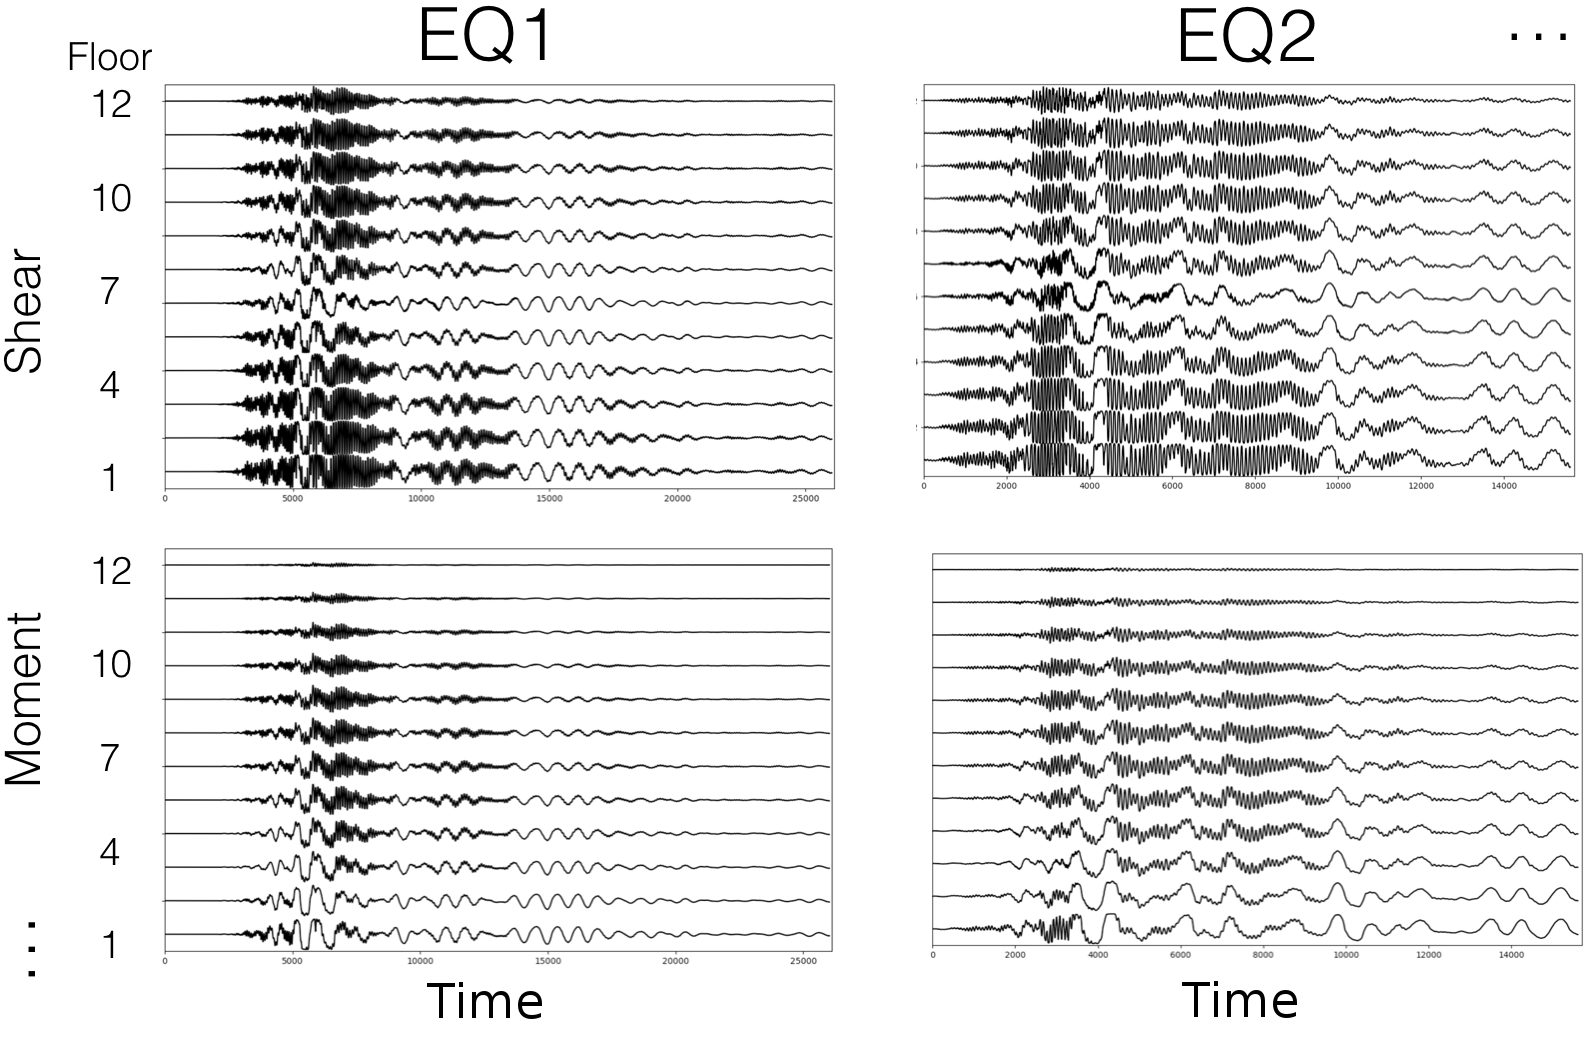
\includegraphics[width=\columnwidth]{figs/structure} 
	\caption{An overview of the data collected by the civil engineers during the simulation. The main challenge in this project is to design visualizations which highlight interesting patterns across the different dimensions, attributes, and scales.}
	\label{fig:data}
\end{figure}

%% This visualization view (right part of Fig. 1) gives users a way to explore the data. It includes three parts: (C) time series plots for the ground acceleration data, (D) a heatmap plot for the time series of the each individual attribute, and (E) a 2D histogram to compare two different physical attributes. These plots can be linked and brushed, such that selecting one region in one plot shows a visualization of the relevant subset in the other plots.

\paragraph*{NLP Model and Probability Product Kernel for cross-earthquake comparisons}
\label{sec:method}
A different view (left part of Fig. 1) organizes the entire dataset more abstractly. For example, suppose we want to compare the shear value across different earthquakes. Based on the fact and observation that simulation data has periodic features, we use a bag-of-words analogy inspired from Natural Language Processing (NLP). We split each earthquake simulation into a set of segments with a fixed period (P), producing segments that are represented as  $13 \times P$ matrices. After applying the segmentation, each earthquake simulation becomes a set of matrices (the ``words'' in the bag of words, which we call ``motifs''). For any two motifs coming from two earthquakes (of possibly different periods), we compare them directly as continuous time series, by upsampling the shorter motif to the length of the longer. After representing simulations as motifs, we calculate the similarity between any two earthquake simulations by mapping the set of motifs to a Gaussian distribution in Hilbert space, and use Bhattacharyya's similarity to compare the earthquakes~\cite{conf/icml/KondorJ03}.

%TODO: add formula
\paragraph*{Matrix diagram views}
\label{matrixvis}
We use matrix diagrams to visualize both the behavior across earthquakes, and within an earthquake, and use D3's existing matrix diagram infrastructure. Each cell in the across-earthquake matrix represents the similarity between two entire simulations using Bhattacharyya's measure, as described above. In this view, users can select cells in order to show a more detailed comparison of one single earthquake against another (or even against itself), comparing all motifs in one earthquake to all motifs in the other. These two views allow users to explore interesting finding. For example, in Fig. 1A, the eleventh earthquake is clearly quite dissimilar to all other earthquakes (as evidenced by the mostly-white row of values).

%\begin{figure*}[h]
% \centering 
% 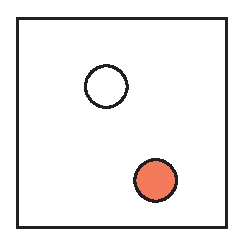
\includegraphics[width=\textwidth]{figs/sample} 
% \caption{Double Column Figure.}
% \label{fig:sample2}
%\end{figure*}

